\rev{
\section{Technique Summary}

To give a better overview of all the techniques introduced in section \ref{sec:software} and \ref{sec:hardware}, we give a brief summary in this section to see how these techniques contributes to FPGA based NN accelerator design. Each technique is judged from two aspects: how it affects hardware design and to which level it relates to NN models. Figure~\ref{fig:summary} shows the summary. 

\begin{figure}[ht]
    \centering
    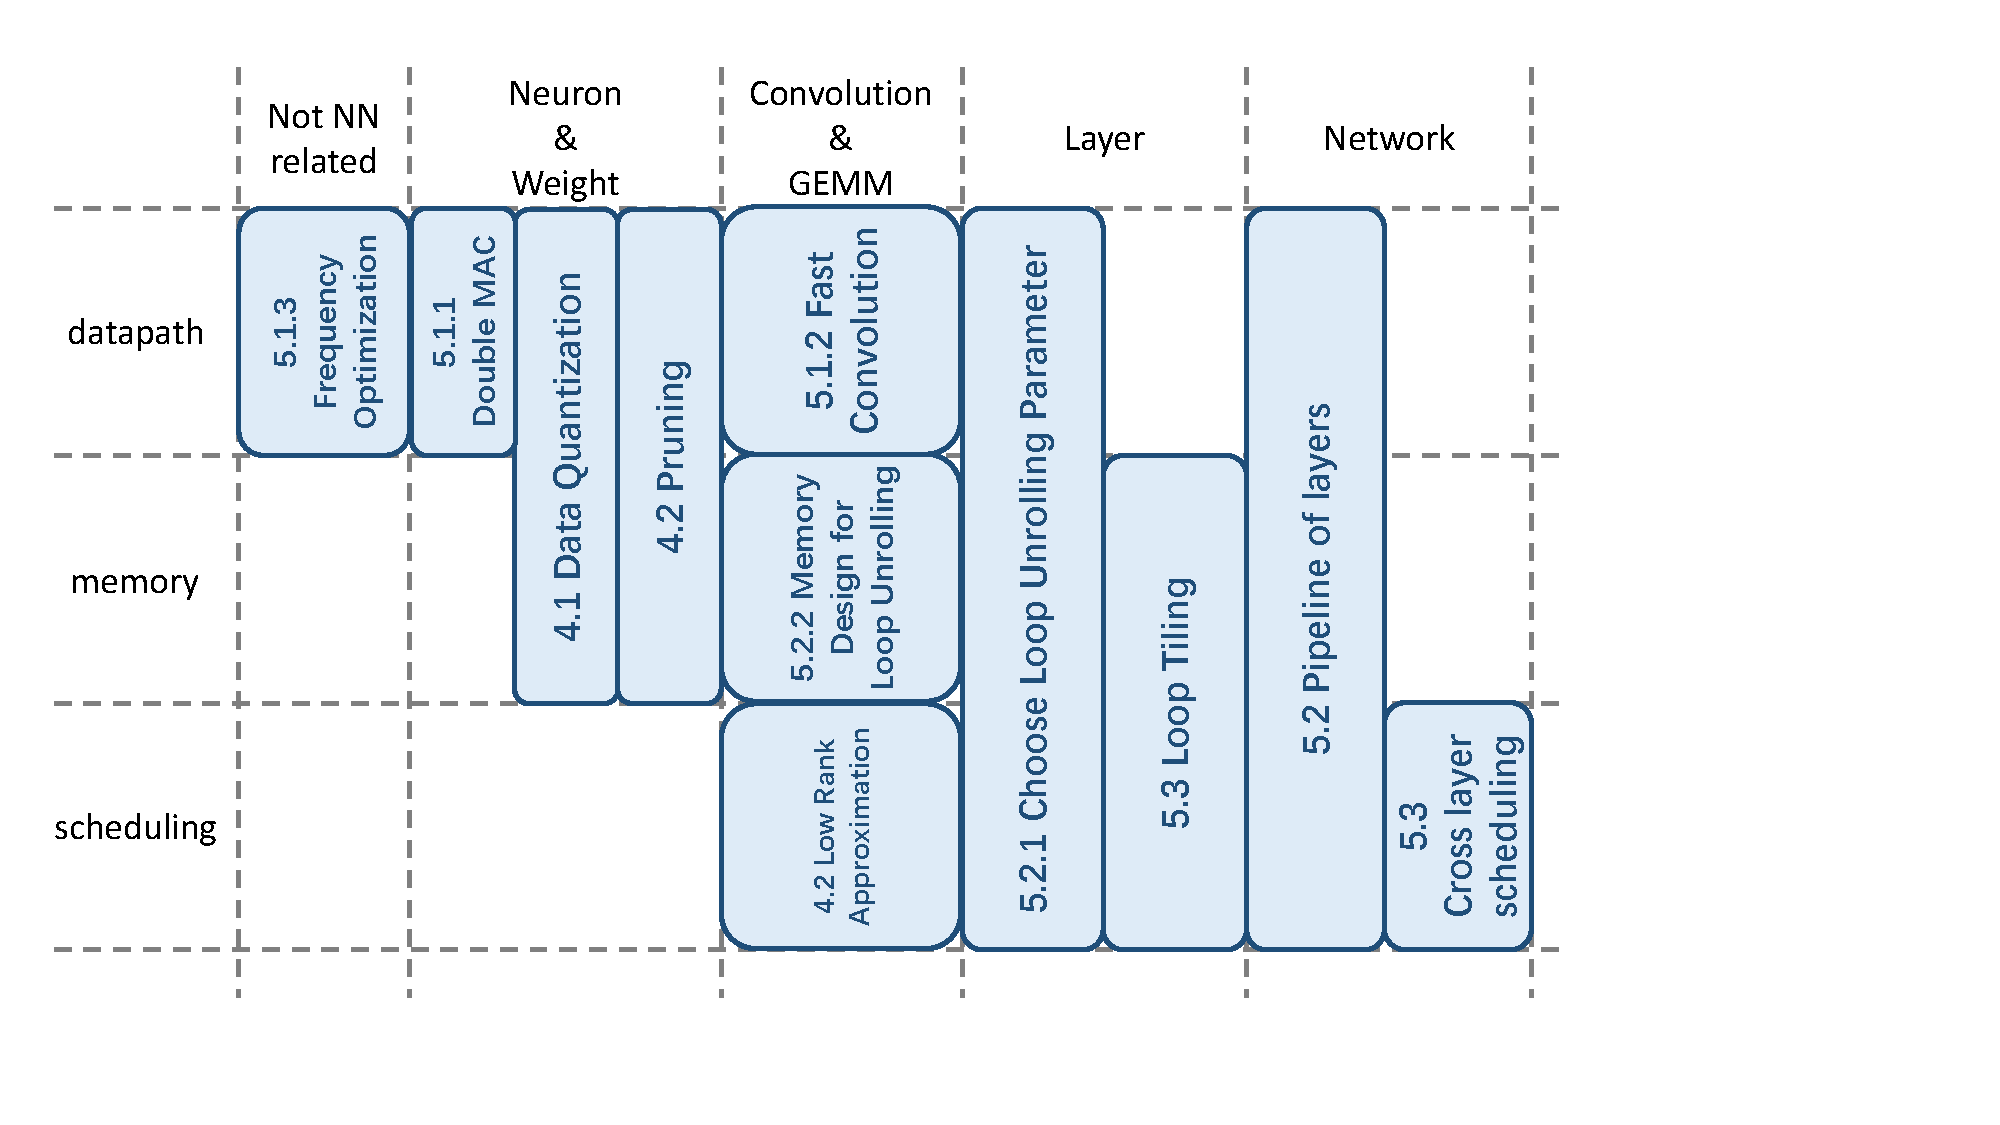
\includegraphics[width=0.8\columnwidth]{fig/summary.pdf}
    \caption{A brief summary of both the software and hardware techniques in section \ref{sec:software} and \ref{sec:hardware}.}
    \label{fig:summary}
\end{figure}

A hardware design basically consists of three parts: datapath, memory, and scheduling. Existing techniques have covered NN model features from single neuron level to the whole network level. From the figure, we see that the more we focus on higher level of NN model feature, the less we can do with datapath and the more we can do with scheduling and memory design. 

Much of the techniques lies in the neuron level and the convolution level. There are two reasons for this phenomena. The first reason is that few feature can be utilized in layer level and network level. Most of the existing NN models introduce a simple structure with cascaded layers~\cite{krizhevsky2012imagenet,simonyan2014very} or simply adding a by-path~\cite{he2016deep}. New features like depth-wise convolution~\cite{Howard2017MobileNets} and the complex branch in SSD~\cite{Liu2015SSD} may brings more design opportunity. But few work focuses on these models. The second reason is that the scale of an FPGA chip is limited. An FPGA chip usually consists of hunderds to thousands of DSPs. This number is still too small compared with a single neural network layer with more than 100M operations. 

So the chance of future techniques should come from two aspects. The first is the evolution of network structure. The second is the scaling up of FPGA based system, with larger chips or multiple chips.
}